\chapter{Resultados}

En este capítulo se recogen los resultados más relevantes de la optimización de Hiperparámetros
\section{Optimización del Máximo Error de Validación}
En esta sección se encuentran los resultados de las optimizaciones realizadas teniendo en cuenta únicamente el máximo error de validación
\subsection{Conjunto pequeño: Comparación de métodos}


\begin{figure}[h!]
\centering
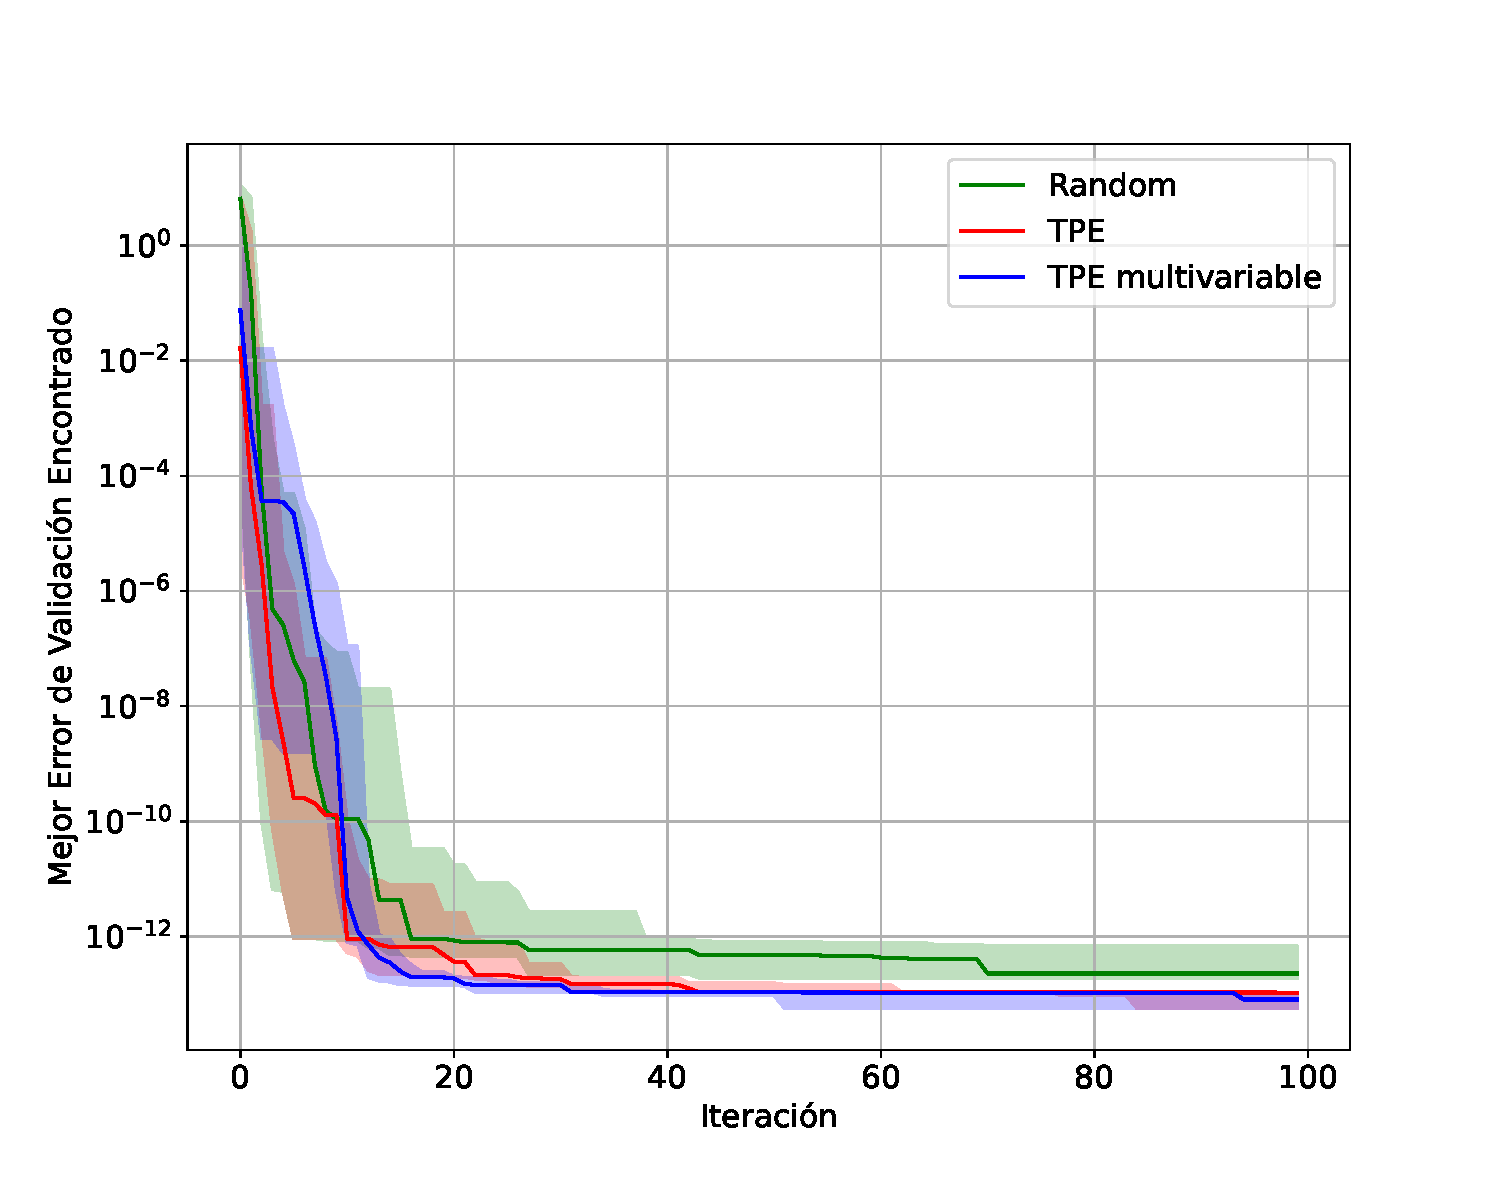
\includegraphics[width=.9\columnwidth, trim={1cm, 1cm, 1cm, 1.1cm}]{benchmark_0.pdf}
\caption{Comparación de convergencia. Se muestran los cuartiles para 20 optimizaciones realizadas, en cada caso.}
\label{fig:bench0}
\end{figure}

Utilizando un conjunto de entrenamiento con cien ondas equidistantes en el espacio del parámetro unidimensional $q: 1 < q < 8$, se quiere optimizar el error de representación para un conjunto de validación con quinientas ondas (cinco veces más denso). Los hiperparámetros a optimizar son $\textbf{x} = (n_{max}, l_{max}, \hat{\Lambda}_0)$, dejando $\varepsilon$ fijo en $1\times 10^{-12}$ para simplificar la búsqueda, que se realiza en los siguientes intervalos:

\begin{align*}
n_{max} &\in \{5, 6, 7, ..., 20\},\\
l_{max} &\in \{1, 2, 3, ..., 10 \},\\
\hat{\Lambda}_0 &\in \{q_0 \ | \ q_0 = 1 + i \Delta q, \ i\in \mathbb{N} : 0 \le i \le 99, \ \Delta q = 7/99 \}.
\end{align*}

Son 16 valores de $n_{max}$, 10 valores de $l_{max}$ y 100 para $q_0$ ($\hat{\Lambda}_0 = q_0$). Lo que hace un total de 16000 combinaciones posibles.

En la figura \ref{fig:bench0} se puede ver el resultado de realizar 20 optimizaciones de 100 iteraciones con tres diferentes métodos; búsqueda aleatoria (\textit{random}), TPE y TPE multivariante (los tres métodos están implementados en Optuna \cite{optuna_2019}). En linea oscura se representa la media del mejor error a cada iteración, y la zona sombreada representa los cuartiles. Aparte, en linea de trazo se marca el mejor error obtenido realizando una búsqueda exhaustiva (\textit{grid search}).


En las primeras 10 repeticiones los tres métodos son equivalentes, pues para el algoritmo TPE (tanto el normal como el multivariante) se parte de un muestreo aleatorio de 10 observaciones. En la figura \ref{fig:bench0} se ve claramente que luego de las décima iteración se produce el cambio más notorio entre los tres métodos. Gráficamente se puede ver que ambas versiones del algoritmo TPE dan un mejor resultado que la búsqueda aleatoria, pero aparte de esto se pueden utilizar métricas como el \textbf{mejor valor encontrado} para la mediana de $y$ o el \textbf{área bajo la curva} o \textbf{AUC} (\textit{Area Under the Curve})\cite{Dewancker2016ASF}. En la tabla \ref{tab:comp1} están los resultados de estas métricas, considerando solo las últimas 90 iteraciones.


\begin{table}
\centering
\begin{tabular}{@{}lccc@{}}
\toprule
\textbf{Algoritmo} & AUC (Mediana) & Mejor $Mediana(y)$ encontrada \\ 
\midrule
Búsqueda Aleatoria & $2.59\times 10^{-10}$ & $2.26\times 10^{-13}$ \\ 
TPE & $1.20\times 10^{-11}$ & $1.04\times 10^{-13}$ \\ 
TPE Multivariante & $5.20\times 10^{-12}$ & $5.48\times 10^{-14}$ \\ 
\bottomrule
\end{tabular} 
\caption{Comparación entre algoritmos de optimización.}
\label{tab:comp1}
\end{table}

\subsubsection*{Búsqueda Exhaustiva}
La búsqueda exhaustiva o \textit{grid search} consiste en probar todas las combinaciones posibles dentro de un espacio de hiperparámetros para seleccionar la solución óptima. Es decir que si se quiere buscar la combinación óptima de $(n_{max}, l_{max})$ para un rango de valores $n_{max} \in N,$ $l_{max} \in L$ se deberán probar todas las combinaciones posibles del producto cartesiano $N \times L = \{(n_{max}, l_{max}) | n_{max} \in N, l_{max} \in L\}$. 

\begin{figure}[h!]
\centering
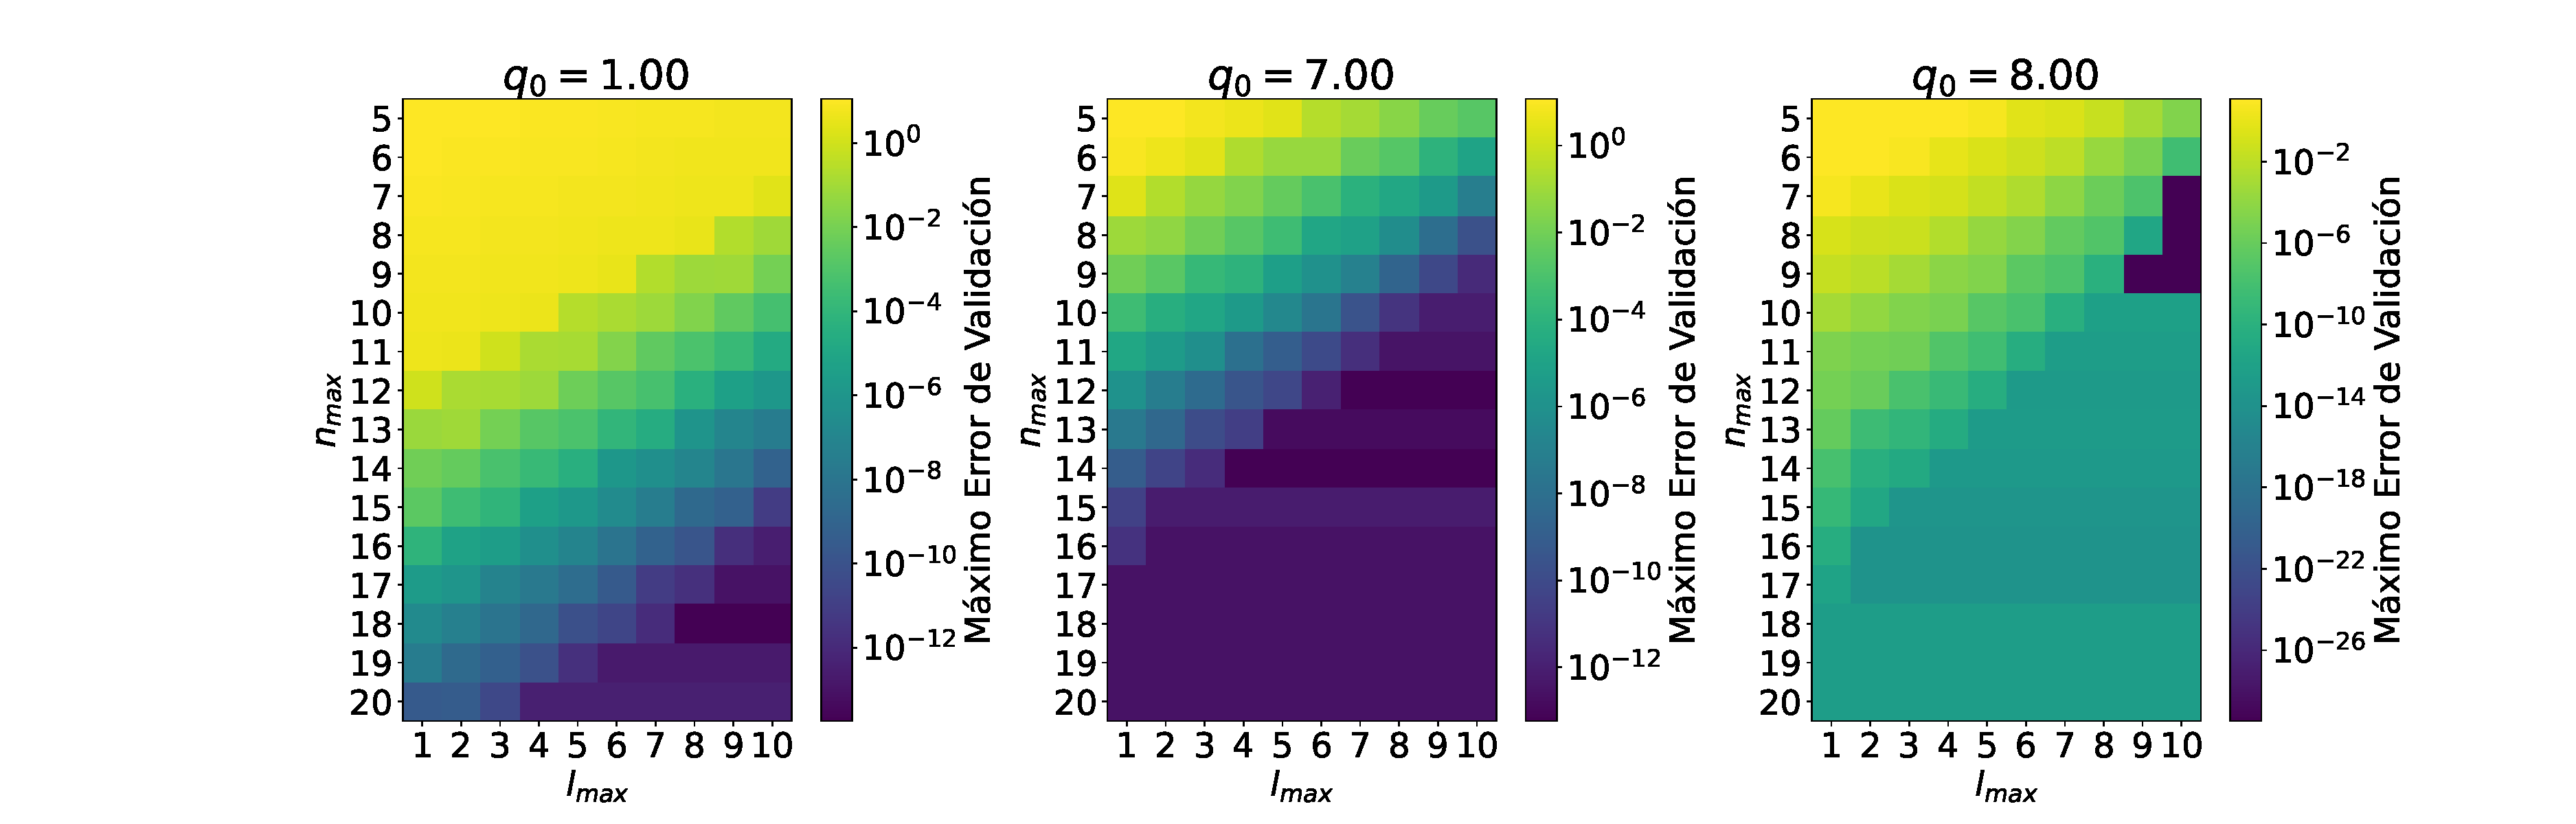
\includegraphics[width=1.05\columnwidth, trim={8cm, 1cm, 5cm, 1.1cm}]{grid_3_seeds.pdf}
\caption{Máximo error de validación en función de $n_{max}$ y $l_{max}$ para tres diferentes semillas $q_0$. }
\label{fig:grid_3_seeds}
\end{figure}

\begin{figure}[h!]
\centering
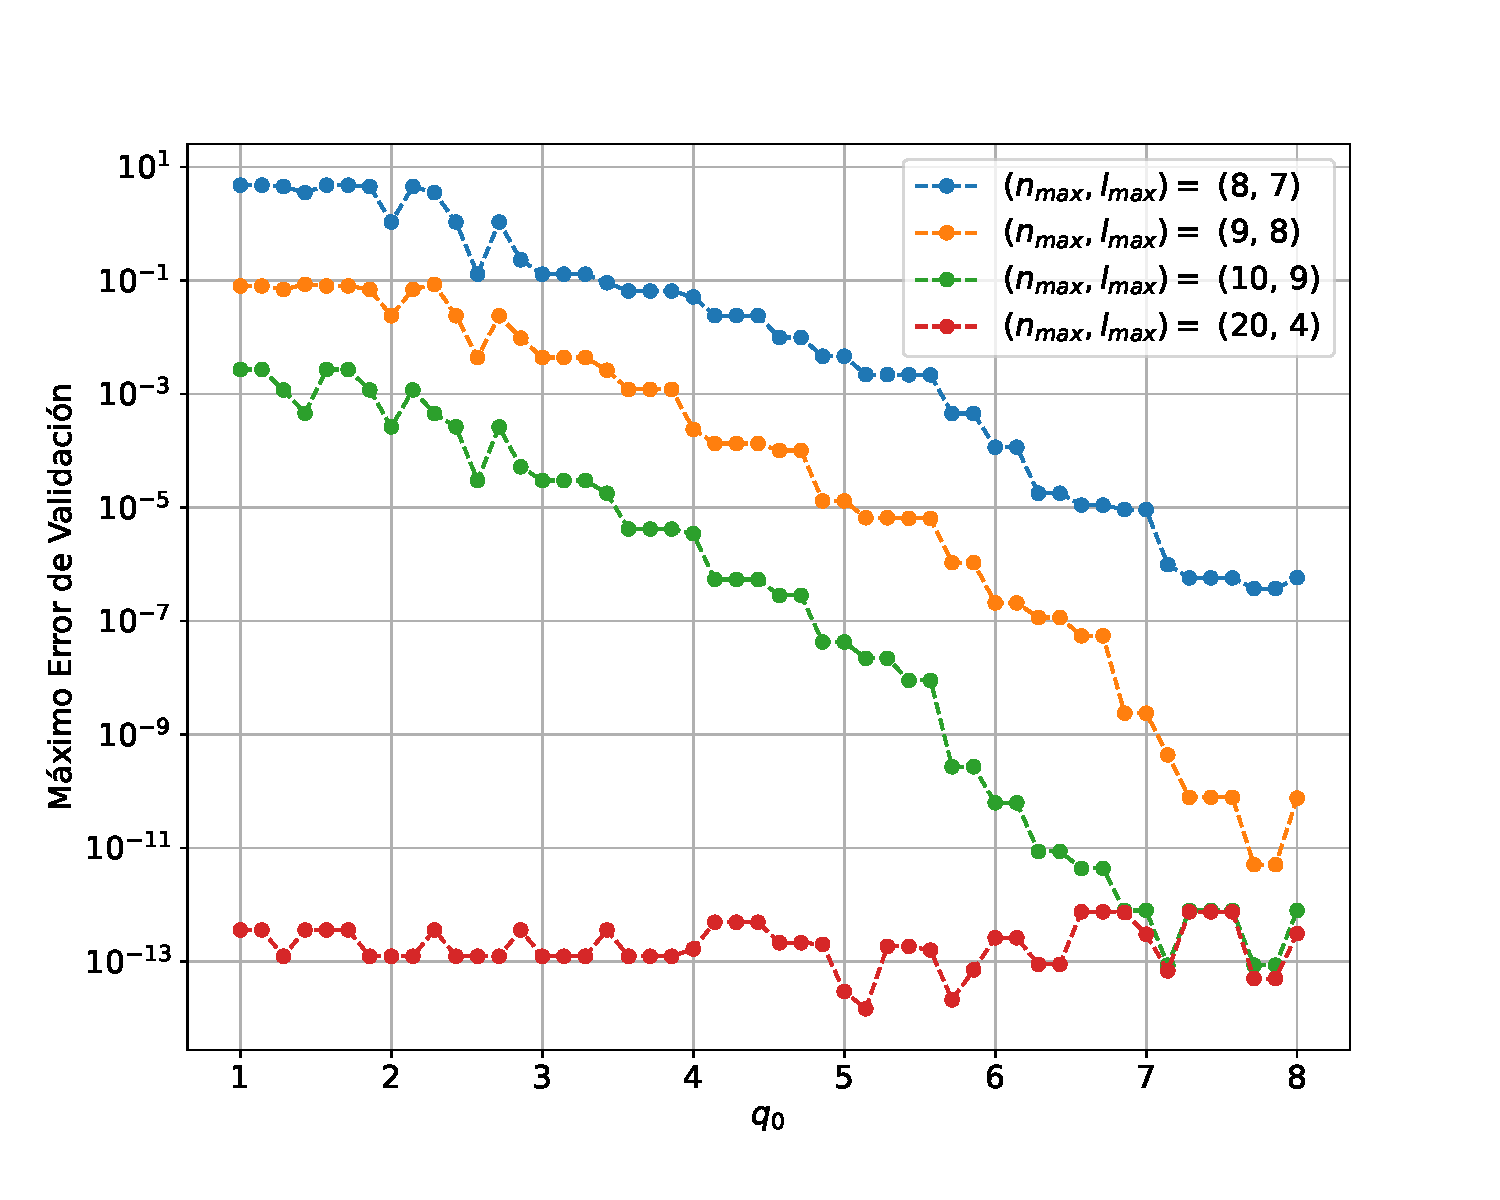
\includegraphics[width=.8\columnwidth, trim={1.1cm, 1cm, 1cm, 1.2cm}]{grid_seeds_0.pdf}
\caption{Máximo error de validación en función de la semilla $q_0$ para distintas combinaciones de $(n_{max}, l_{max})$}
\label{fig:grid_seed_0}
\end{figure}


 
%La ventaja de este método está en que el resultado óptimo está garantizado, pues se pueden comparar todos los resultados entre sí y elegir el mejor. El problema es que, como se mencionó, la función $f$ es costosa de evaluar, y por otro lado el número de combinaciones posibles escala exponencialmente con cada hiperparámetro extra a optimizar (además se debe tener en cuenta que la semilla $\hat{\Lambda}_0$ tendrá generalmente más de una dimension).

%Por estas razones la búsqueda exhaustiva no será un método viable en la mayoría de los casos que son de interés para este trabajo. Sin embargo se puede poner a prueba con casos simplificados para luego comparar los resultados con otros métodos más eficaces.

Si bien no se puede graficar el error en función de los tres hiperparámetros a la vez, se puede obtener bastante información al dejar fijo uno o dos hiperparámetros. Por ejemplo en la figura \ref{fig:grid_3_seeds} se observa el error de validación en función de las combinaciones posibles de  $n_{max}$ y $l_{max}$ para tres diferentes semillas. 

Luego en la figura \ref{fig:grid_seed_0} se ven los resultados de variar únicamente la semilla para diferentes combinaciones de $n_{max}$ y $l_{max}$. 
En este conjunto de datos se observa que para $(n_{max}, l_{max})=(20, 10)$ hay una diferencia de 9 ordenes de magnitud entre la peor y la mejor semilla (datos en color verde). Sin embargo para $(n_{max}, l_{max})=(15, 10)$ la diferencia es de 13 ordenes de magnitud (datos de color azul). Además el valor óptimo de la semilla no coincide exactamente en estos dos ejemplos, aunque tengan un comportamiento similar. Es decir que la influencia de la semilla depende del resto de hiperparámetros, sobre todo se tiene que tener en cuenta que en este caso la tolerancia \textit{greedy} tenía un valor $\varepsilon = 1\cdot 10^{-12}$, por lo que no se va a obtener un resultado mucho mejor que este.

\begin{figure}[h!]
\centering
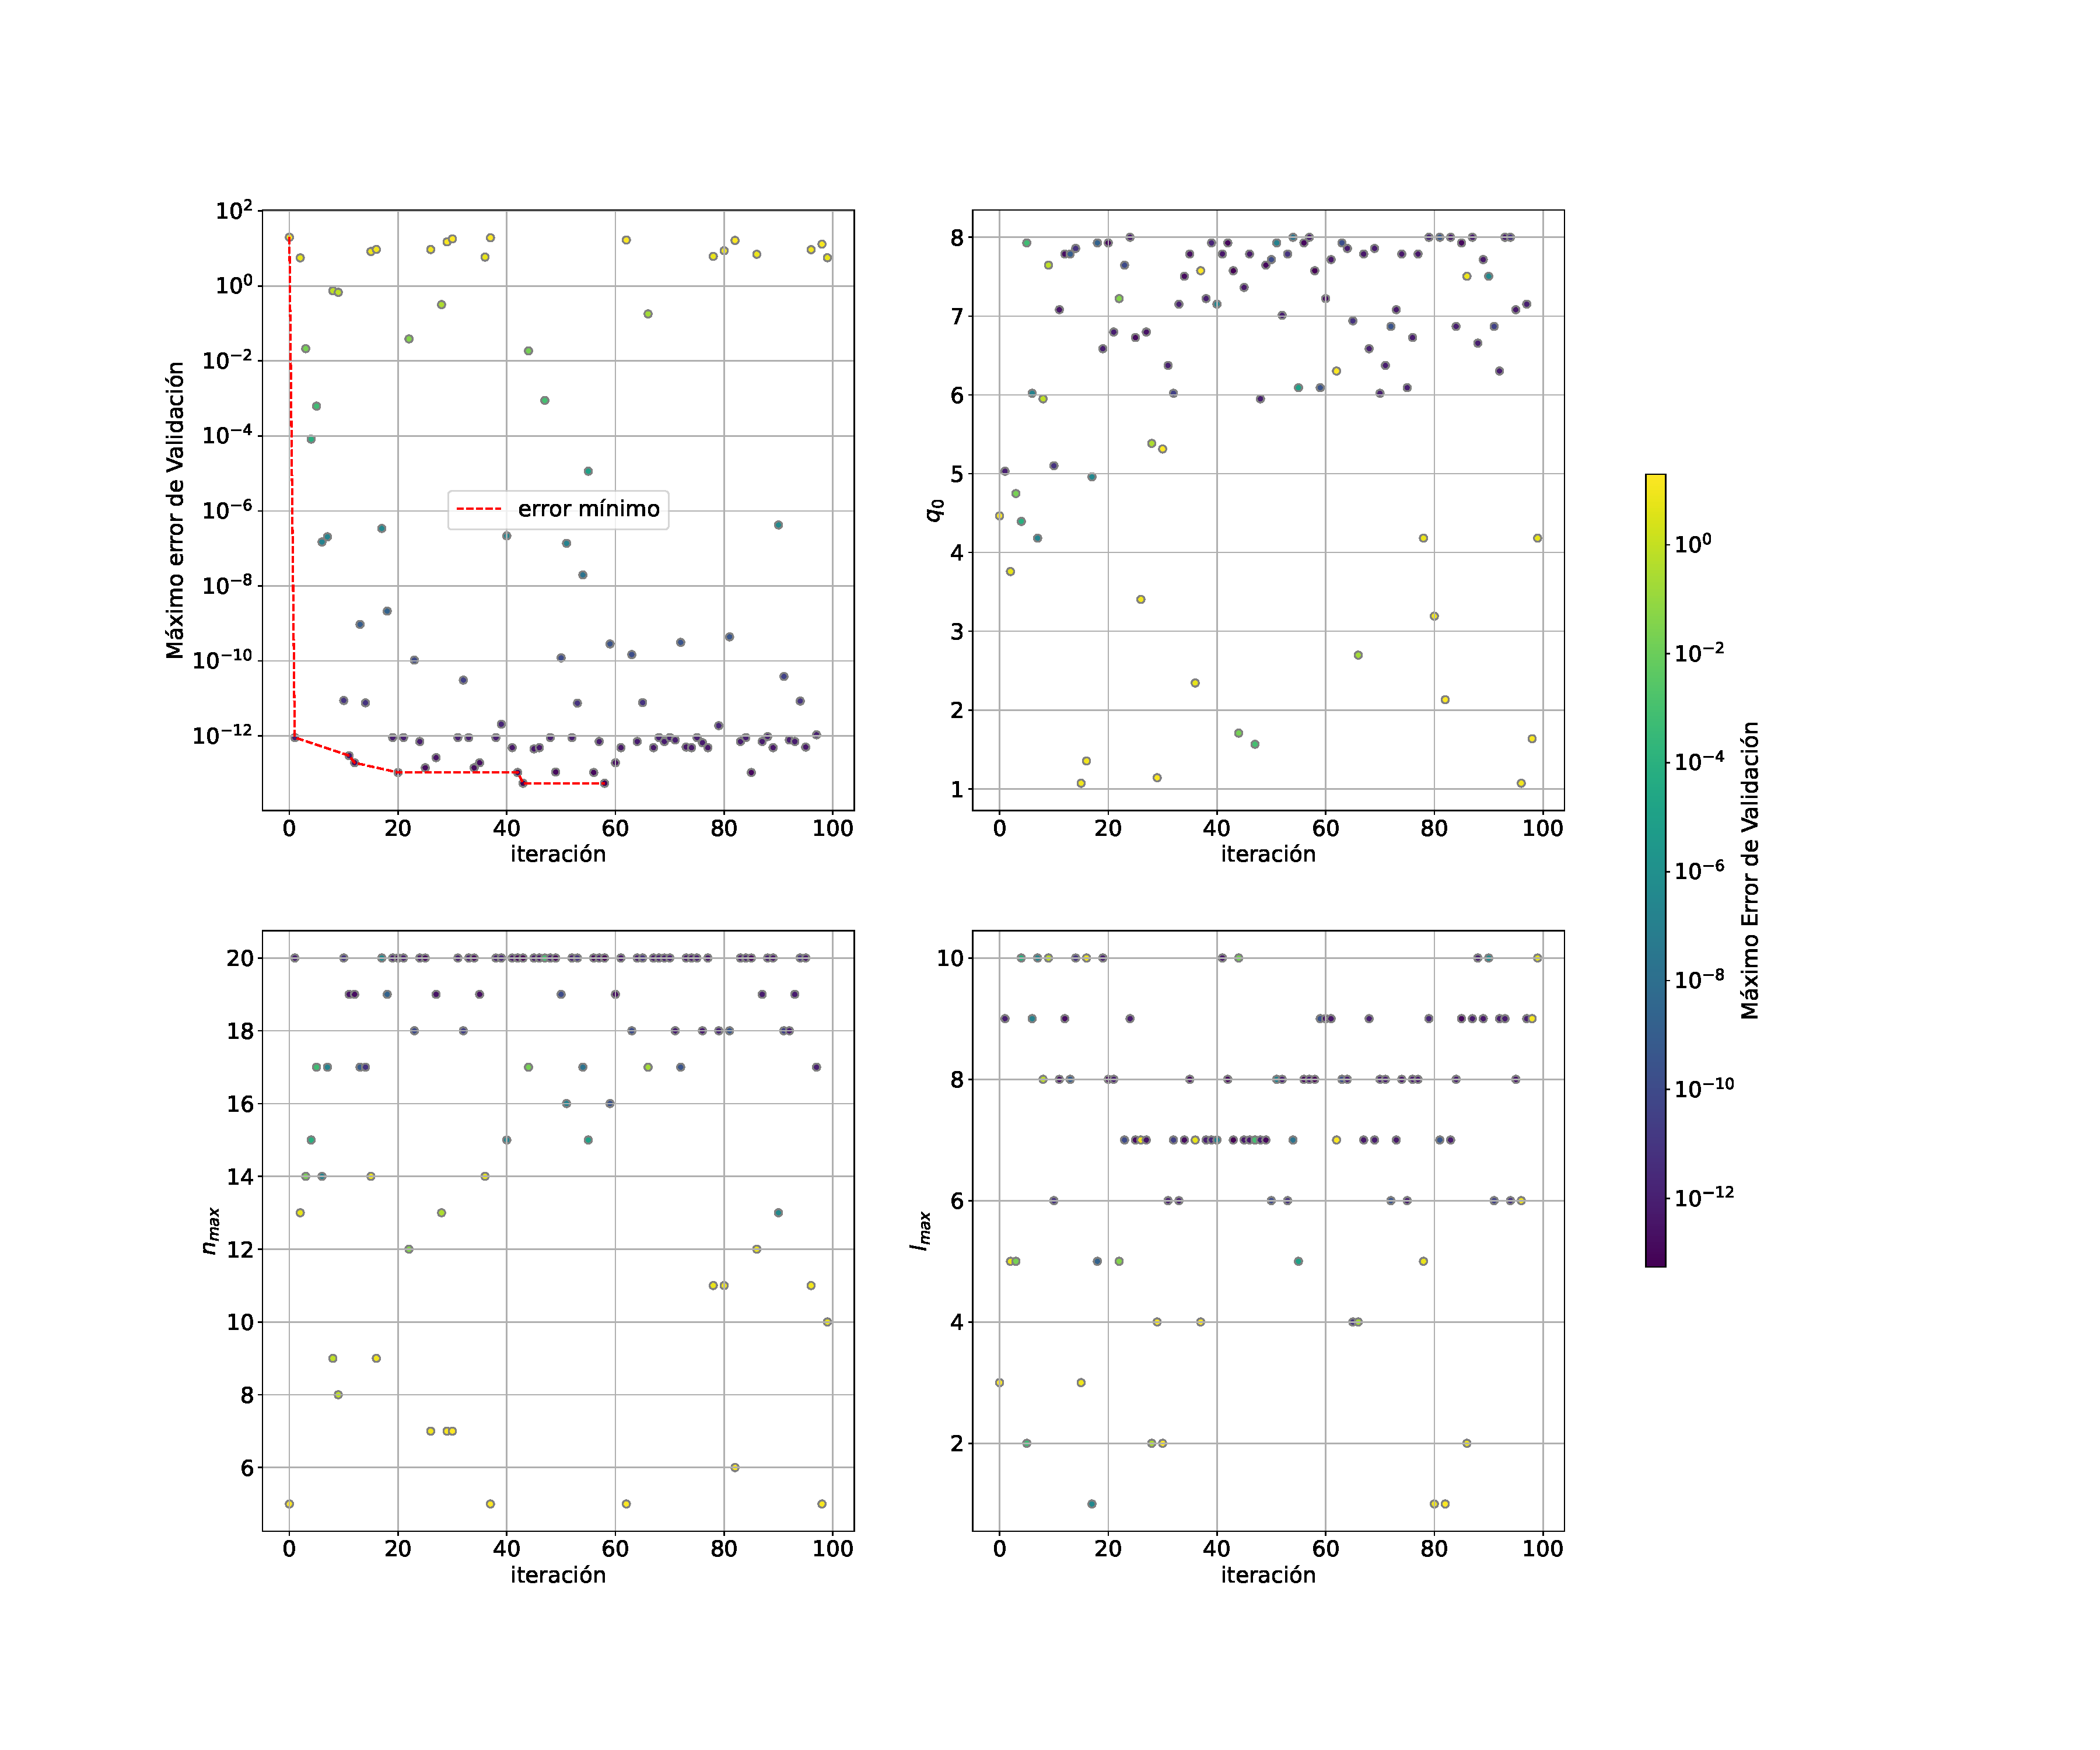
\includegraphics[width=1\columnwidth, trim={5cm, 5cm, 11cm, 5cm}]{Optuna_1d_simple.pdf}
\caption{Optimización con 100 iteraciones utilizando el algoritmo TPE multivariante para el conjunto de entrenamiento con semilla unidimensional.}
\label{fig:optuna_1d}
\end{figure}

\subsubsection*{Tiempo de Optimización}

Si bien la búsqueda exhaustiva garantiza encontrar el mejor resultado posible dentro del espacio de búsqueda, el tiempo necesario para realizar la búsqueda hace que el método no sea aplicable a casos relativamente complejos. En este caso sencillo, con 16000 combinaciones, la búsqueda requirió \textbf{25 horas} para completarse. En cambio las optimizaciones realizadas utilizando los algoritmos TPE tardaron una media de \textbf{8 minutos}.

Por último en la figura \ref{fig:optuna_1d} se puede ver gráficamente el proceso de optimización utilizando el algoritmo TPE multivariable.

\subsection{Optimización Completa}

\begin{figure}[p!]
\centering
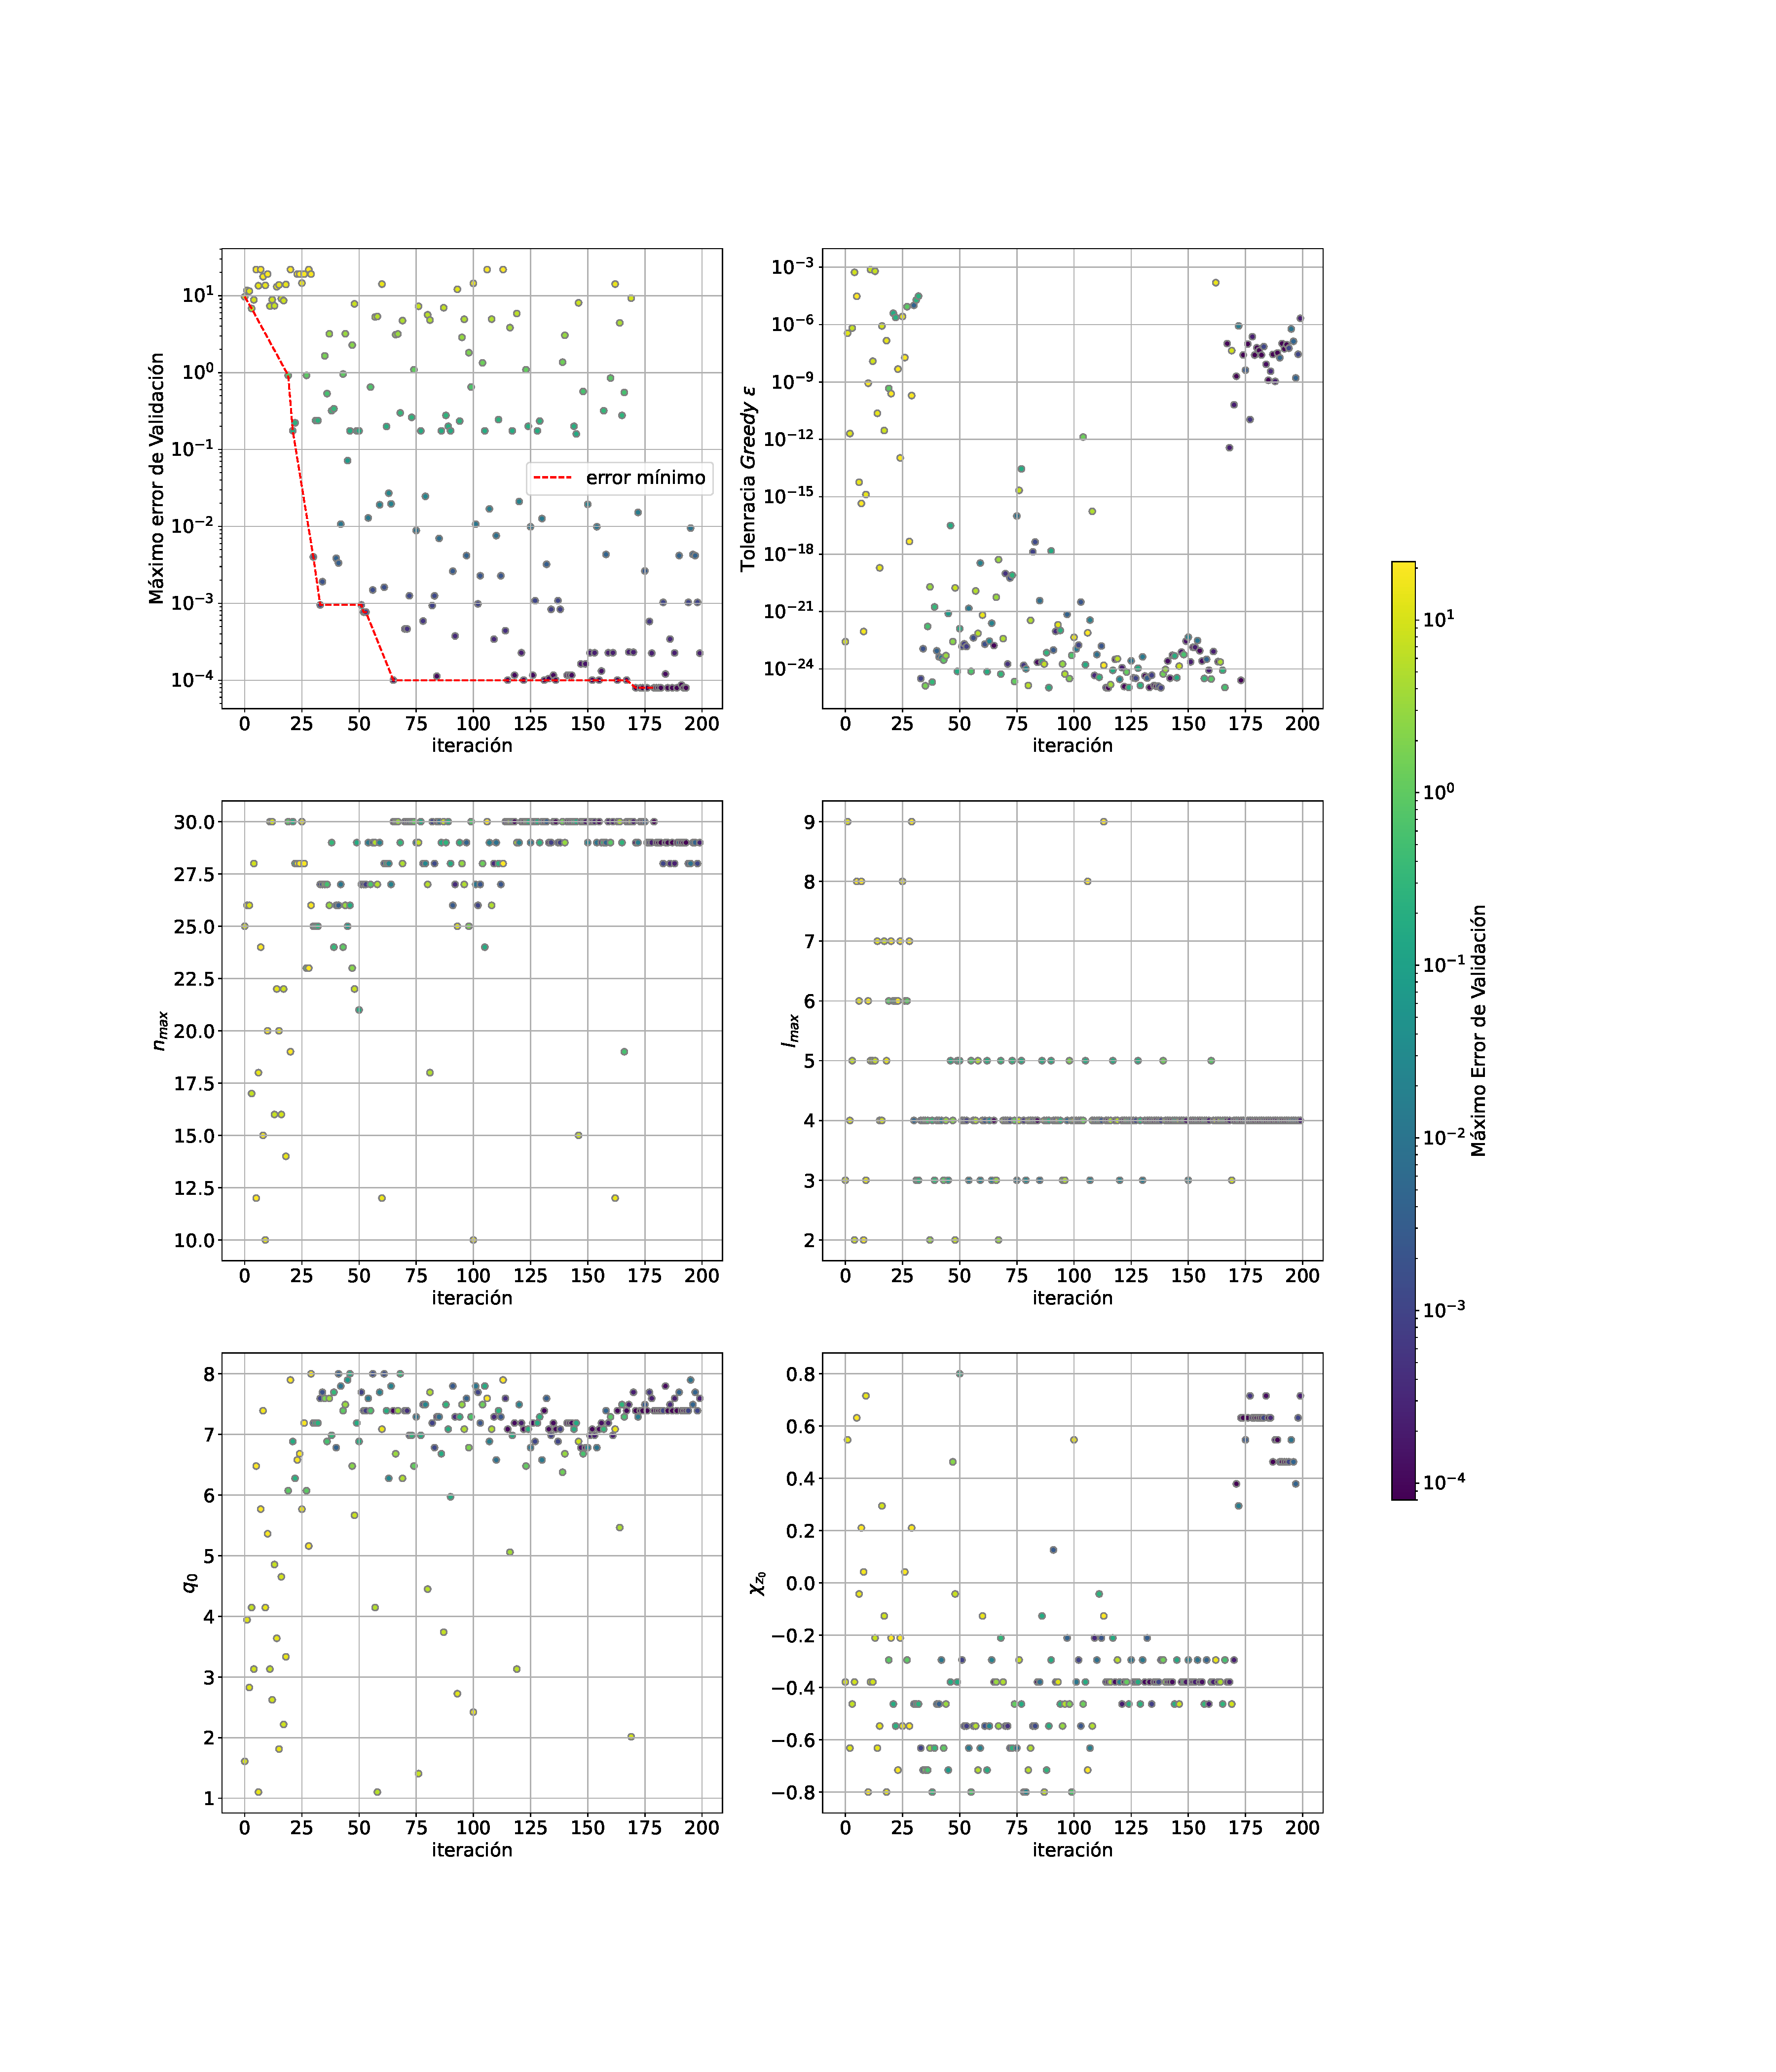
\includegraphics[width=1\columnwidth, trim={6cm, 5cm, 12cm, 5cm}]{Optuna_2D.pdf}
\caption{Optimización con 500 iteraciones para semilla de dos dimensiones utilizando el algoritmo TPE Multivariante con 4 trabajadores en paralelo.}
\label{fig:optuna_2d}
\end{figure}

Utilizando un conjunto de entrenamiento con 70 valores discretos de $q$ equidistantes en el rango [1, 8] y 20 de $\chi_z$ ($\chi_{z_1} = \chi_{z_2}$) en el rango [-0.8, 0.8], dando lugar a un total de 1400 funciones de onda, se muestran los resultados de optimizar el máximo error de validación utilizando un conjunto de validación con 100 valores para $q$ y 30 valores para $\chi_z$ con un total de 3000 funciones de onda.

La optimización se realizó en el siguiente espacio de búsqueda:
 
\begin{align*}
n_{max} &\in \{10, 11, 12, ..., 60\},\\
l_{max} &\in \{2, 3, 4, ..., 20 \},\\
\varepsilon &\in \{ 10^{-20}, 10^{-19}, 10^{-18}, ..., 10^{-4}\},\\
Q_0 &= \{ q_0 \ | \ q_0 = 1 + i \Delta q, \ i\in \mathbb{N} : 0 \le i \le 69, \ \Delta q = 7/69 \},\\
X_0 &= \{\chi_{z_0} \ | \ \chi_{z_0} = -0.8 + j \Delta \chi_z, \ j\in \mathbb{N} : 0 \le j \le 19, \ \Delta \chi_z = 1.6/19 \}, \\
\hat{\Lambda}_0 &\in \{ (q_0, \chi_{z_0}) \ | \ q_0 \in Q_0,\ \chi_{z_0} \in X_0 \}.
\end{align*}

En este caso hay más de 23 millones de configuraciones posibles.

En total se realizaron 500 iteraciones, y el mejor máximo error de validación obtenido en la iteración número 269 fue de $1{.}45\times 10^{-6}$ con los hiperparámetros:

\begin{align*}
&n_{max}^* = 59, \\
 &l_{max}^* = 4, \\
&\varepsilon^* = 10^{-17},\\
 &q_0^* = 7.899, \\
 &\chi_{z_0}^* = 0.716.
\end{align*}

En la figura \ref{fig:optuna_2d} se observa la evolución de la optimización realizada, que requirió alrededor de 8 horas para completarse. Se puede ver que para cada hiperparámetro se observa una convergencia a cierto valor, pero sin dejar de lado la exploración, es decir, que se siguen evaluando hiperparámetros fuera del rango que parece óptimo, de forma que se evita caer mucho tiempo en mínimos locales.

\subsubsection*{Estimación Tiempo de Búsqueda Exhaustiva}

Teniendo en cuenta que una optimización con 500 iteraciones se realiza en aproximadamente 8 minutos, se puede estimar el tiempo que sería necesario para realizar una búsqueda exhaustiva o \textit{grid search} en este espacio de búsqueda con 23 millones de configuraciones posibles.

\begin{equation}
t_{grid\ search} \approx \frac{23\ millones\ de\ configuraciones \cdot 8 hs}{500\ configuraciones} = 368000\ hs
\end{equation}

El resultado sería aproximadamente unas 368 mil horas, o 42 años de cómputo necesarios para realizar la búsqueda exhaustiva. Es decir que en este caso la búsqueda exhaustiva no es una opción a considerar.

Ahora, teniendo en cuenta que una iteración del algoritmo TPE es más costosa que entrenar y evaluar la base (pues en TPE además se modelan las distribuciones de probabilidad), este tiempo realmente sería menor, pero con un factor muy cercano a 1, por lo que las conclusiones de este resultado siguen siendo válidas.

\subsubsection*{Error de Prueba}

Luego de realizar la optimización se puede utilizar un conjunto de prueba, es decir, un conjunto de elementos que no se usaron para el entrenamiento ni para la optimización, para poner a prueba el resultado obtenido.

En este caso, utilizando un conjunto de prueba con 6000 elementos como resultado de un muestreo de 150 valores para $q$ y 40 para $\chi_z$, se calculó el máximo error relativo, siendo:

\[
error \ relativo = \frac{\| h_{\lambda} - P_n h_{\lambda} \|^2}{\| h_{\lambda} \|^2}
\]

Como resultado, se obtuvo un máximo error relativo de $3.84 \cdot 10^{-7}$.



\subsubsection{Importancia de los Hiperparámetros}

Una vez realizada una optimización se puede estimar la importancia relativa de cada hiperparámetro con el algoritmo fANOVA \cite{pmlr-v32-hutter14}. Básicamente la idea es dividir la varianza total en distintos componentes que representen la varianza producida por cada hiperparámetro. En la figura \ref{fig:param_import} se observa a la izquierda en naranja los resultados para la optimización realizada, y a la derecha en azul se ven los resultados para otro espacio de búsqueda, esta vez con $n_{max} \in \{20, ..., 30\}$  y $l_{max} = \{2, ..., 8\}$ (es decir que se redujo el espacio de búsqueda para $n_{max}$ y $l_{max}$). Se puede ver que la importancia que tienen los hiperparámetros depende claramente del espacio de búsqueda, pero en general se observó que $n_{max}$ y $l_{max}$ suelen tener mayor importancia relativa al resto de hiperparámetros.

\begin{figure}[h!]
\centering
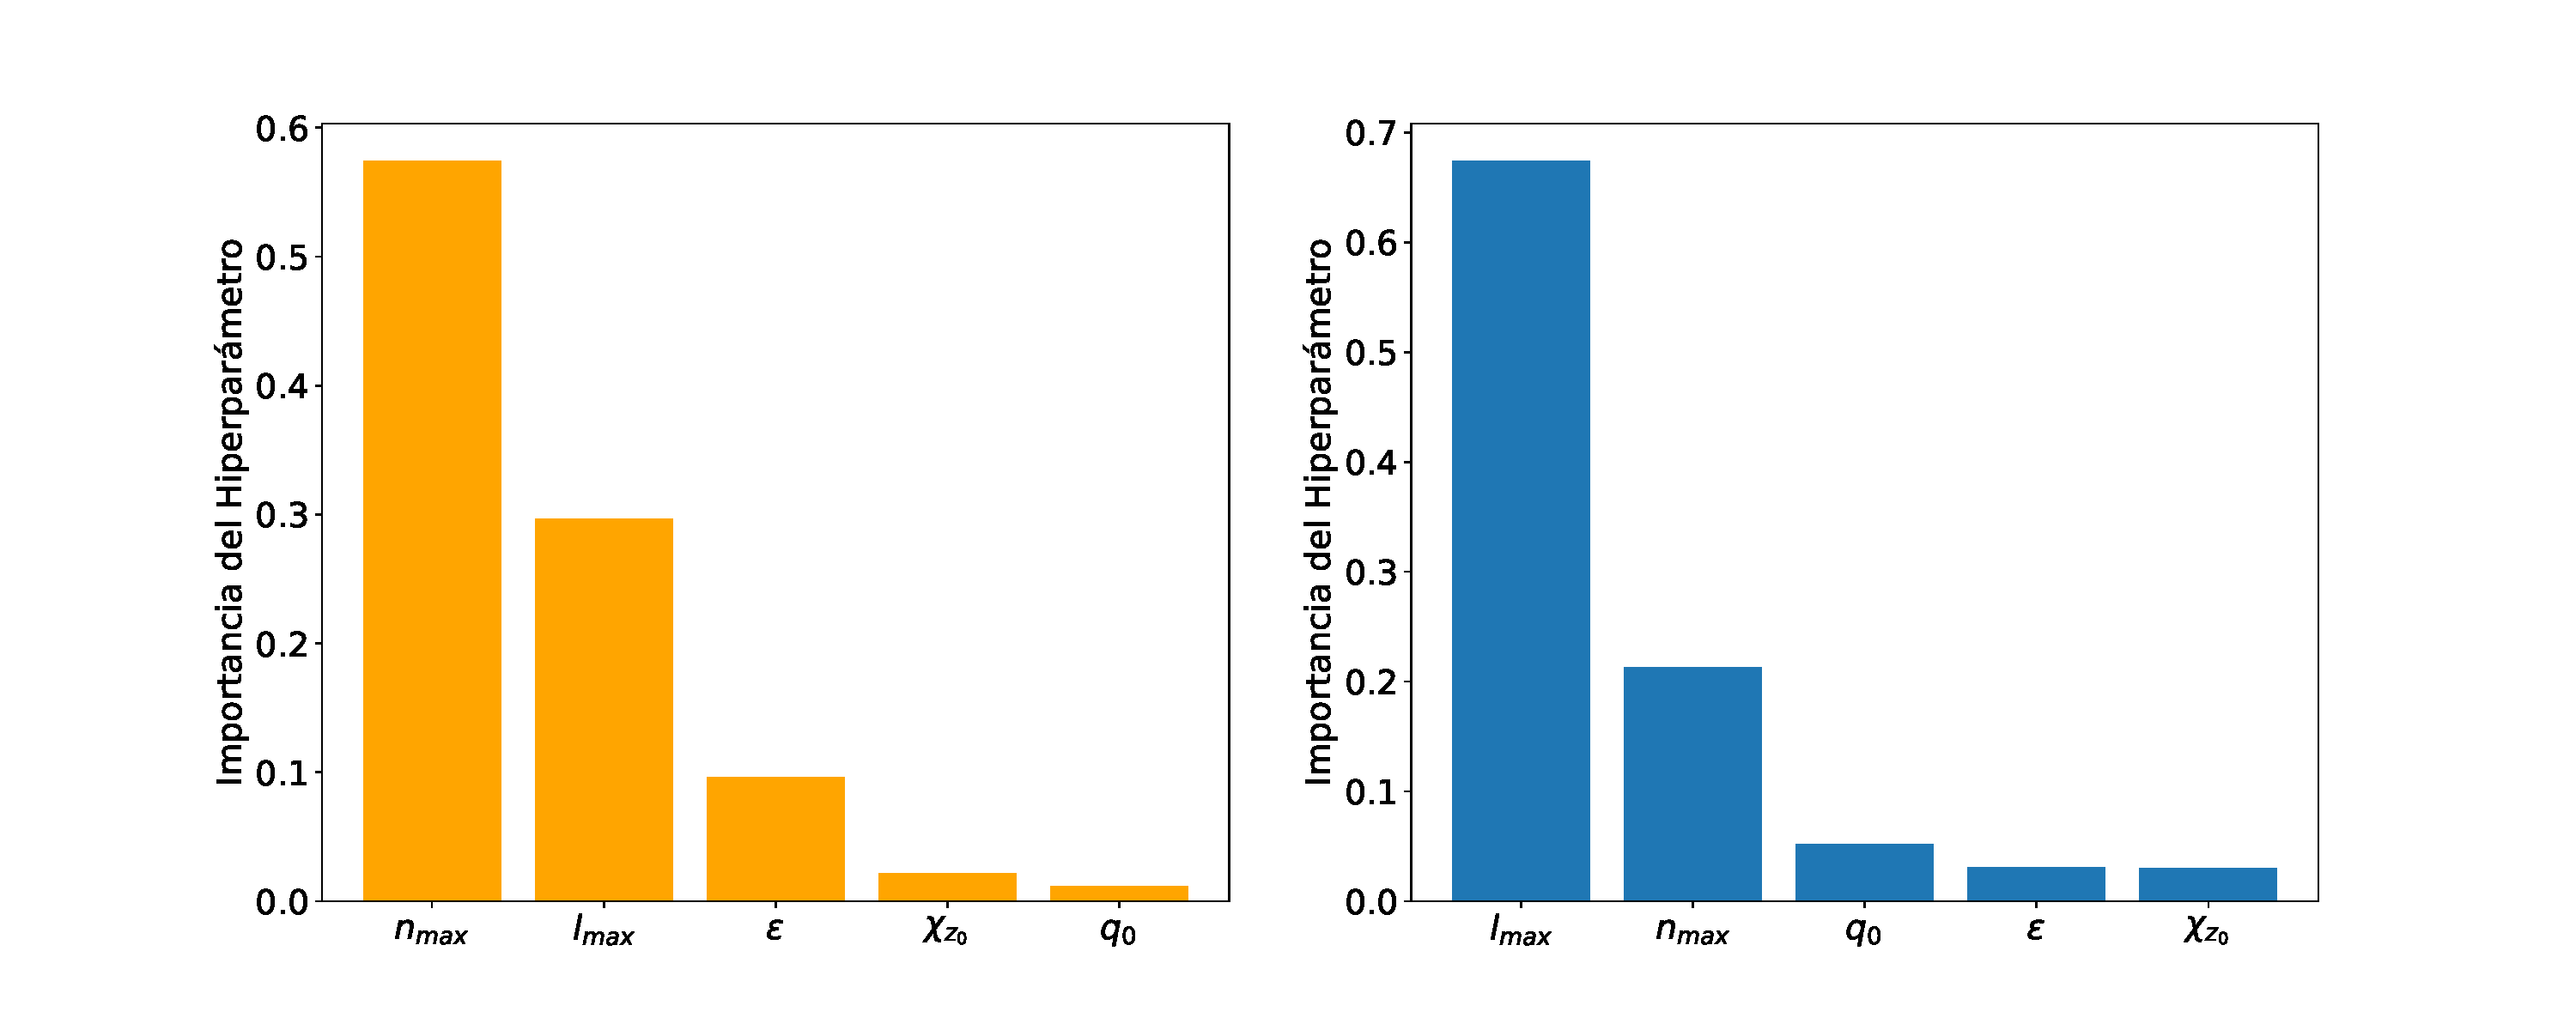
\includegraphics[width=1\columnwidth, trim={5cm, 2cm, 5cm, 2cm}]{params_importance_full.pdf}
\caption{Importancia relativa de los hiperparámetros para dos espacios de búsqueda diferentes. $n_{max}$ y $l_{max}$ suelen ser los hiperparámetros más importantes en la mayoría de los espacios de búsqueda.}
\label{fig:param_import}
\end{figure}



\newpage
\section{Optimización Multiobjetivo}

En esta sección se encuentran los resultados más relevantes de la optimización multiobjetivo, que optimiza el máximo error de evaluación al mismo tiempo que el tiempo necesario para proyectar el conjunto de validación a la base creada.


\subsection{Frente de Pareto}

Utilizando un conjunto de entrenamiento con mil funciones de ondas equidistantes en el espacio del parámetro unidimensional $q: 1 < q < 8$, y un conjunto de validación diez veces más denso (diez mil funciones de onda) se optimizó $\textbf{x} = (n_{max}, l_{max},\varepsilon, \hat{\Lambda}_0)$, en los siguientes intervalos:

\begin{align*}
n_{max} &\in \{10, 11, 12, ..., 20\},\\
l_{max} &\in \{1, 2, 3, ..., 10 \},\\
\varepsilon &\in \{  10^{-20}, 10^{-19}, 10^{-18}, ..., 10^{-6}\}, \\
\hat{\Lambda}_0 &\in \{q_0 \ | \ q_0 = 1 + i \Delta q, \ i\in \mathbb{N} : 0 \le i \le 999, \ \Delta q = 7/999 \}.
\end{align*}

Una buena forma de visualizar los resultados es graficando ambos objetivos a la vez. En la figura \ref{fig:pareto} cada punto representa una observación, y lo interesante de este gráfico es que puede observar fácilmente el frente de Pareto (en color naranja). El frente de Pareto está conformado por aquellas observaciones que no sean dominadas por ninguna otra, pero son incomparables entre sí, por lo que este conjunto reemplaza a $\textbf{x}^*$. Una vez obtenido este conjunto se debe elegir que objetivo es más importante y seleccionar una configuración $\textbf{x}$ dentro del conjunto de Pareto.

\begin{figure}[h!]
\centering
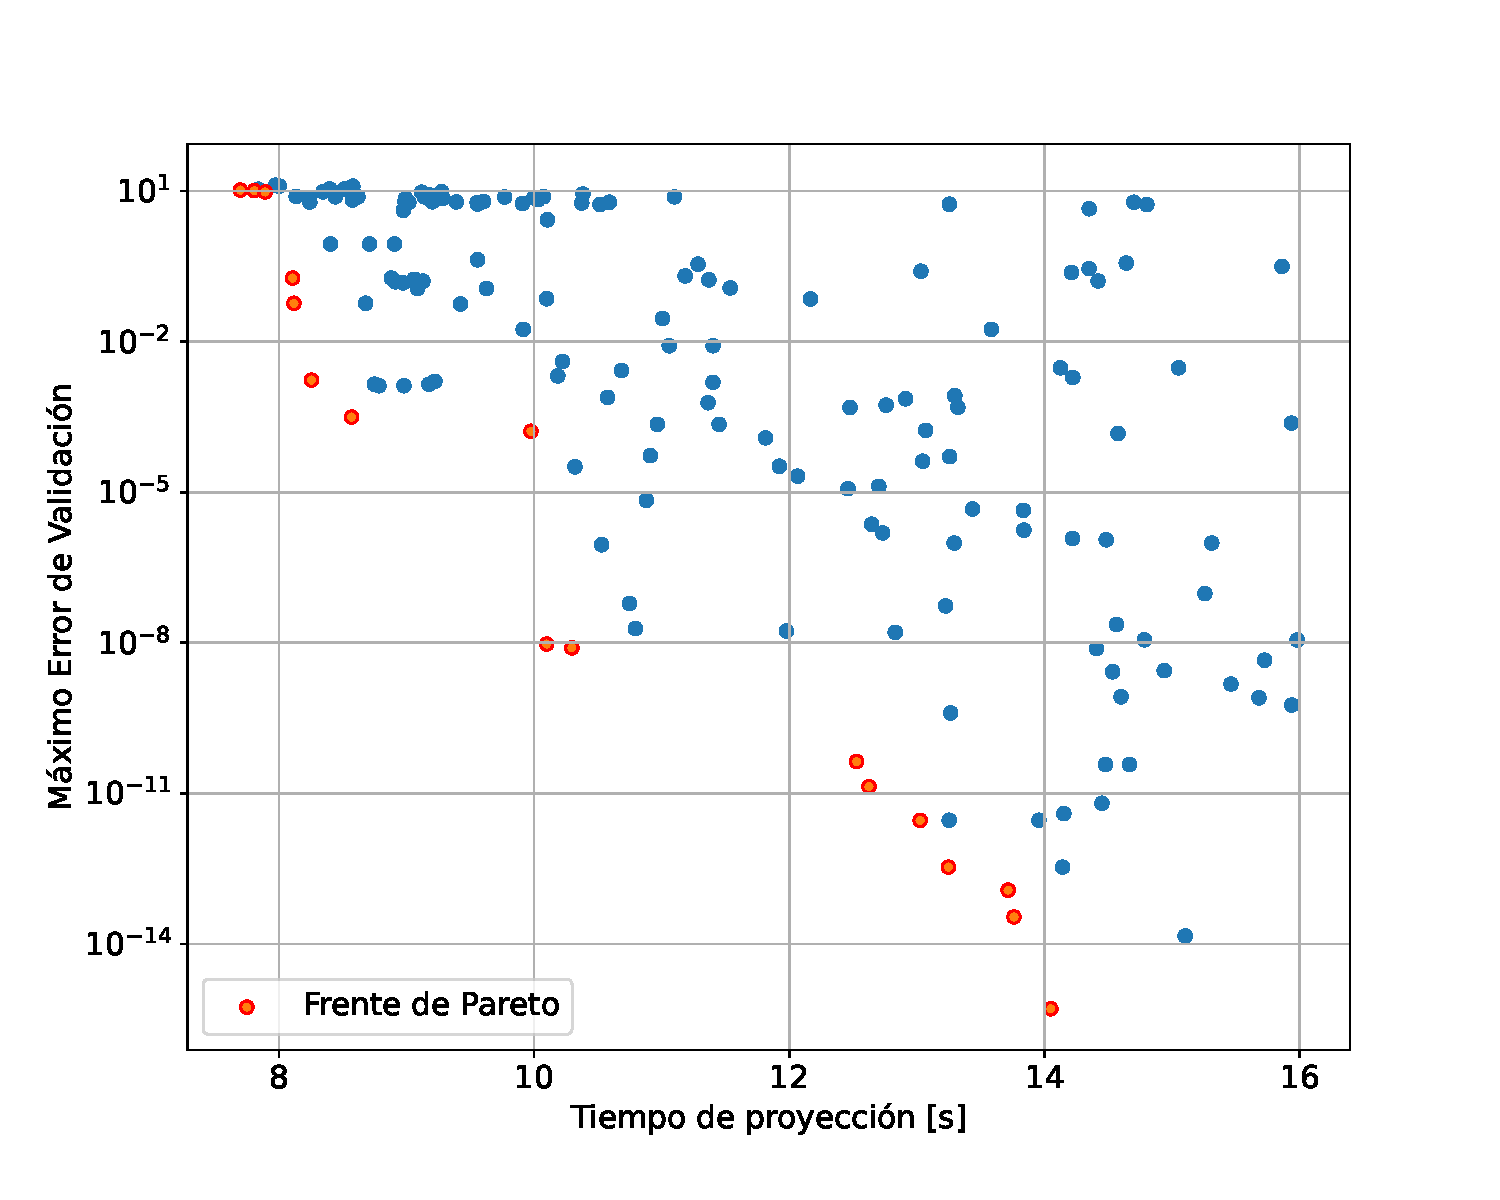
\includegraphics[width=.8\columnwidth, trim={1cm, 1cm, 1cm, 1cm}]{motpe_pareto.pdf}
\caption{Máximo error de validación versus el tiempo de proyección. Cada punto representa una observación. En color naranja se marca el frente de Pareto.}
\label{fig:pareto}
\end{figure}

\subsection{Tiempo de Proyección versus Hiperparámetros}
\label{sec:corr_t}

\begin{figure}[p]
\centering
\includegraphics[width=1\columnwidth, trim={5cm, 2cm, 5cm, 2cm}]{motpe_correlation.pdf}
\caption{Relación entre el tiempo de ejecución y los diferentes hiperparámetros para una optimización de 160 iteraciones.}
\label{fig:motpe_param_rel}
\end{figure}


La optimización multiobjetivo resulta muy interesante, pero en el contexto de ondas gravitacionales, se observa que hay una gran dependencia entre el tiempo de proyección y $n_{max}$. Mas bien, como ya se observó en la figura \ref{fig:t_vs_nmax} de la sección \ref{sec:hp-gw} sobre bases reducidas \textit{hp-greedy}, el tiempo de proyección depende casi exclusivamente del valor de $n_{max}$, siempre que el conjunto de entrenamiento sea lo suficientemente denso \mbox{($n_{max} \cdot 2^{l_{max}} < N$).}

En la figura \ref{fig:motpe_param_rel} se puede ver la dependencia entre los diferentes hiperparámetros y el tiempo de proyección en segundos, para las observaciones realizadas. Claramente hay una tendencia bastante lineal al considerar $n_{max}$.

Para entender la dependencia entre $n_{max}$ y el tiempo de proyección hay que recordar la ecuación \eqref{eq:coefs} de los coeficientes $c_{i, \lambda}$:

\[
c_{i, \lambda} = \langle e_i, h_{\lambda} \rangle .
\]

Para proyectar una función de onda $h_{\lambda}$ a una base reducida se deben calcular los coeficientes $c_{i, \lambda}$, y el número de coeficientes será igual al número de elementos de la base $\{  e_i\}$. Por lo tanto mientras más elementos tengan las bases locales, mayor será el tiempo de proyección.
